%%%%%%%%%%%%%%%%%%%%%%%%%%%%%% Preamble 
\documentclass[titlepage]{scrartcl} 
\usepackage{amsmath,amssymb,amsthm,fullpage} 

\usepackage{graphicx} % support the \includegraphics command and options
\usepackage{caption}
\usepackage{subcaption}
\usepackage{pdfpages}

\begin{document}
\pagestyle{plain}
\pagenumbering{arabic}

%%%%%%%%%%%%%%%%%%%%%%%%%%%%%% Heading 
	\title{EE/CS 52 SoPC Digital Oscilloscope}
	\subtitle{Technical Manual}
	\author{Santiago Navonne} 
	\date{Spring 2014} 
	\maketitle
	
%%%%%%%%%%%%%%%%%%%%%%%%%%%%%% Table of Contents

	\tableofcontents
	\clearpage


%%%%%%%%%%%%%%%%%%%%%%%%%%%%%% Body
	\section{Introduction}
	This document describes the system workings and details of the EE/CS 52 System-on-Programmable-Chip (SoPC) Digital Oscilloscope.\\

	The guide describes first the hardware, and then the software, giving for both a system overview, followed by a detailed description of every part of the system. In Appendix~\ref{original}, the schematics and printed circuit board used in the original prototype can be found.

%%%%%%%%%%%%

	\section{Hardware}
	This section explains how the system's hardware works, from the system overview to the detailed description of each element. The interactions of components are described, and detailed schematics, timing diagrams, and board layouts are provided.
	
	\subsection{System Overview \label{sec:overview}}
	The highest level illustration of the structure of the system is provided in the block diagram of Figure~\ref{fig:main_blocks}. The parts colored blue are created within the FPGA component (\textit{U2}), while the parts colored red are outside components.\\

	\begin{figure}[h!]
	\vspace{-4cm}
	\centerline{\includegraphics[width=29cm, angle=90, origin=c]{img/block_diagram.pdf}}
                	\caption{Highest level block diagram of the SoPC Oscilloscope system. The diagram is described in Section~\ref{sec:overview}.}
               	\label{fig:main_blocks}
	\end{figure}
	
	The central component of the system is the NIOS II CPU, a soft-core device generated within the FPGA. A NIOS II/e processor is used upon power-up, and can be upgraded to the faster NIOS II/s by connecting the device to a computer. Within the NIOS CPU are included the chip select decoding and interrupt control logic sections. The chip select decoding logic uses the address bus to activate the chip select control line of the device being accessed, if it requires one. The interrupt controller processes interrupt control signals from hardware devices and makes them available to software procedures.\\

	The display controller, also included within the FPGA, controls the VRAM serial clock and all of the display timing signals, updating the VRAM serial data bus as needed to ensure that data is correctly shown on the display. The debouncers and decoders take signals from the user input sections of the system (i.e. rotary encoders and push-button switches), and process them to translate them into interrupt signals for the processor. These signals are accessed through a Parallel IO (PIO) interface. The triggering logic is configured through a PIO interface, and reads the signal output by the ADC, determining the correct moment to trigger based on triggering mode, level, slope, and delay parameters. The component then instructs the FIFO to start writing samples as necessary. The First-In First-Out (FIFO) data structure stores samples to be processed by the CPU. The FIFO starts being filled when instructed by the trigger, and once full transmits this signal to both the trigger, which disables the trigger signal, and the CPU, which goes ahead and processes the samples.\\

	Outside the FPGA but closely related is the reset logic, which generates a reset signal for the NIOS CPU on power-up, power failure, and when requested by the user. Similarly, the clock logic is an outside component that generates a constant, 38 MHz clock signal used throughout the system. A JTAG connector and interface is used to program and debug the FPGA and NIOS CPU.\\

	Every signal exiting the FPGA, with the sole exception of the I$^2$C bus, is buffered. These chips provide a layer of protection for the FPGA, as well as more driving power and voltage flexibility for the components being operated.\\

	Four memory devices are used by the system. The Serial Configuration device (EPCS) is used to store the FPGA that is loaded upon start-up. The device uses dedicated serial control signals to communicate with the FPGA. The Static Random Access Memory (SRAM) device is the system's volatile memory, used to store the software's variables, stack, and other uninitialized memory. The device shares the data and address buses with the other memory devices, and is selected and controlled by a small set of exclusive signals from the CPU. The Electrically Erasable Programmable Read-Only Memory (EEPROM) device is the system's non-volatile memory, used to store code and constants. This device also shares the data and address buses with the other memory devices, and it is, too, selected and controlled by a small set of exclusive signals from the CPU. Two Video RAM (VRAM) devices are used as a buffer for the frames being shown on the display. Data is put there by the CPU via the VRAM controller, and subsequently extracted serially and shown on the LCD by the display controller. This device shares the data bus with other memory devices, while the address bus is exclusive from the controller to the device. A set of VRAM specific control signals is also exclusive to this device.\\

	The display is controlled by timing signals from the display controller, which, synchronized with the VRAM controller, ensure that pixels are output over a dedicated bus between display and VRAM at the right moment to be shown in the correct region of the display.\\

	An Analog Front-End (AFE) scales and shifts signals from the oscilloscope probe as needed to prepare them for input into the Analog-to-Digital Converter (ADC). This device, in turn, reads the samples and converts them into digital values, which are then directly relayed to the triggering logic and FIFO within the FPGA. The ADC is also clocked by a control signal routed through the FPGA.\\

	Two rotary encoders with momentary push-button switches provide the user-input interface of the system: the devices are connected to the FPGA and then the decoders and debouncers, which filter process the signals before making them available to the CPU. Finally, a touch screen controller, currently unimplemented, communicates with the CPU over an I$^2$C bus and a dedicated interrupt line used to identify touch screen events. This line is made available to the CPU through a PIO interface. The controller uses an analog interface to drive and read the touch screen.\\
	
	All these elements, after being designed in detail and their connections finalized, are physically placed on a printed circuit board. The front of the board is illustrated in Figure~\ref{fig:pcb}, where each section is highlighted in a different color: the FPGA and related components are colored red; the buffers are green; the memory devices are yellow; the power supply circuitry is blue; the analog interface is orange; the display connector is pink; and the rotary encoders are brown. The components without any highlighting are prototyping and debugging holes and pins, unused in the final design. The back of the board is shown in figure \ref{fib:pcb_back}. Note that no components other than capacitors and resistors are placed on the back of the board, and thus nothing is highlighted.\\

	\begin{figure}[h!]
	\vspace{-2cm}
	\centerline{\includegraphics[width=28cm, angle=90, origin=c]{img/pcb.pdf}}
		\vspace{-2cm}
                	\caption{Front side of the system's Printed Circuit Board (PCB). The color each section is highlighted in identifies the corresponding block.}
               	\label{fig:pcb}
	\end{figure}

	\begin{figure}[h!]
	\vspace{-2cm}
	\centerline{\includegraphics[width=28cm, angle=90, origin=c]{img/pcb_back.pdf}}
		\vspace{-2cm}
                	\caption{Back side of the system's Printed Circuit Board (PCB). Note that this side is only used for routing and placement of passive parts, such as resistors and capacitors.}
               	\label{fig:pcb_back}
	\end{figure}

	The memory map of the system is shown in figure \ref{fig:memory_map}. The \textit{JTAG} device is used for debugging purposes the; \textit{trig\_period}, \textit{trig\_level}, \textit{fifo\_data}, \textit{fifo\_full}, \textit{fifo\_delay}, and \textit{trig\_ctrl} are parallel IO devices used to interface with the triggering logic. Each of these locations in memory contains several registers necessary for the interface to function. \textit{pio\_0} is another parallel IO device, this time used to interface with the rotary encoders and push buttons. Finally, \textit{ram}, \textit{rom}, and \textit{vram} are the memory devices described above. Note that only memory devices have assigned chip select signals, since the other components do not require them; furthermore, note that the VRAM chip select signal does not exist in hardware external to the FPGA.

	\begin{figure}[h!]
	\includegraphics[width=\textwidth]{img/memory_map.png}
                	\caption{Memory map of the system within the NIOS processor, with associated chip select lines and addresses.}
               	\label{fig:memory_map}
	\end{figure}

	\clearpage

	\subsection{FPGA \label{sec:fpga}}
	An Altera EP3C25Q240 Cyclone III Field Programmable Gate Array (FPGA), \textit{U2}, is the central unit of the system. The component and its associated parts are at the center of the PCB, highlighted in red in Figure~\ref{fig:pcb}. Its connections at a system's level are illustrated in the schematic of Figure~\ref{fig:fpga_schematic}. The device is programmed and debugged through a JTAG interface. After debugging, the final design is loaded upon power-on from the serial memory device \textit{U4} through lines \textit{DATA0} and \textit{DATA1}, clocked by \textit{DCLK} and configured through \textit{nCSO}; the debugging and design loading configuration is determined by the MSEL jumpers \textit{JP2}, \textit{JP3}, and \textit{JP4}. Pins 100 and 103 are pulled high through \textit{R1} and \textit{R2} to act as the I$^2$C bus lines \textit{SDA} and \textit{SCL}. Configuration lines \textit{INIT\_DONE}, \textit{CONF\_DONE}, and \textit{nSTATUS} are pulled high, while \textit{nCE} and \textit{CLKUSR} are tied low. Configuration lines \textit{DEV\_OE}, \textit{DEV\_CLRn}, and \textit{nCEO} can be left floating, and are therefore connected to break-out pins in \textit{J3}. Finally, memory selection configuration lines \textit{MSEL2..0} are made available on headers \textit{JP4..2}. For the correct operation of the device, \textit{MSEL2} and \textit{MSEL0} should be jumped on the HI position, while \textit{MSEL1} should be configured to the LO position.\\

	\begin{figure}[h!]
	\vspace{-2cm}
	\centerline{\includegraphics[width=26cm, angle=90, origin=c]{img/fpga_sch.pdf}}
                	\caption{Schematic of the FPGA and related components. Also included are the buffers and power supply. The document is described in Section~\ref{sec:fpga}.}
               	\label{fig:fpga_schematic}
	\end{figure}

	The device contains the system's CPU, as well as all of the logic needed to process analog signals, debounce keys, decode rotary encoders, control the VRAM, and control the display. The logic was designed using the Altera tool chain: Quartus and QSys.\\

	Within the FPGA, several components interact with one another. Figure~\ref{fig:quartus_main} illustrates these components and their interactions.\\

	\begin{figure}[h!]
	\vspace{-4cm}
	\centerline{\includegraphics[width=30cm, angle=90, origin=c]{img/quartus_main.pdf}}
		\vspace{-2cm}
                	\caption{Main block diagram of the FPGA's internal design. The document is described in Section~\ref{sec:fpga}.}
               	\label{fig:quartus_main}
	\end{figure}

	The top left section of the diagram constitutes the user input section. Rotary encoder channels A (\textit{ROT1A}, \textit{ROT2A}) and B (\textit{ROT1B}, \textit{ROT2B}), as well as the push-button lines (\textit{PUSH1}, \textit{PUSH2}), for both devices, are input on pins 57, 63-65, 68, 69. The inputs are processed through debouncers (\textit{DBC1}, \textit{DBC2}) and decoders (\textit{DEC1}, \textit{DEC2}), which filter the signals, generating events as appropriate at their outputs. These events are collected into a bus, that is input to the NIOS processor (\textit{CPU1}) at the \textit{switches\_in} port of \textit{PIO\_0}.\\

	The middle left section of the diagram is the devices triggering logic. The signal from the ADC (\textit{SIG7..0}) is input on pins 9, 13, 18, 21, 37-39, 41; and then connected to the \textit{DATA7..0} input of the triggering block (\textit{TRIG1}). The trigger's general clock (\textit{GCLK}) is connected to the system clock input at pin 31 (\textit{CLK}). All the other lines of the trigger block are connected to their PIO counterpart at the processor. Note that all the control lines (\textit{SLOPE}, \textit{AUTO\_TRIG}, \textit{FIFO\_WE}, \textit{READ}, \textit{RESET}) are collected into a single bus that is then connected to the processor's \textit{trig\_ctrl} PIO interface. The ADC's sample clock on pin 72 (\textit{ACLK}) is clocked at a constant 38 MHz through the system clock (\textit{CLK}).\\

	The bottom left block, \textit{SR1}, is a necessary component for the functioning of the system's serial memory device (\textit{U4}).\\

	In the bottom right, we recognize the VRAM (\textit{VRAM1}) and display (\textit{DISP1}) controllers. These components' inputs are connected to the processor (\textit{CPU1}), with the exception of the interconnected serial row update request (\textit{UREQ}) and acknowledge (\textit{UACK}) signals. The VRAM receives its own dedicated address bus shifted right twice to turn 4-byte addressing into single-word addressing (\textit{vaddr\_out19..2} to \textit{A17..9} and \textit{A8..0}). The dedicated chip select (\textit{CS}) and shared write enable (\textit{WE}) signals are operated as for any other generic controller. All clocks are connected to the system clock. Finally, these two components output all the necessary timing signals for the display and VRAM devices on pins 82, 83, 87, 88, 93-95, 98. Additionally, the VRAM controller output a \textit{RDY} signal, converted to an active-high \textit{WAIT} signal for the processor through inverter \textit{NOT}, to regulate the VRAM access cycles, which use a variable number of wait states.\\

	In the top right, we see the system's NIOS processor (\textit{CPU1}). Apart from the previously described connections, the devices shared address (\textit{ADDR\_BUS18..0}) and data (\textit{DATA\_BUS23..0}) buses for the ROM and RAM devices are output on pins 114, 117-120, 126-128, 131-135, 137, 139, 142, 143, 146-148, 160, 161, 166, 167, 181-189, 194-197, 200-203, 217. The write enable signal (\textit{WE}) is output to the RAM on pin 168, and is also used as the direction signal for the data bus buffers (\textit{U6}, \textit{U9}) on pin 207 (\textit{DATA\_DIR}). The RAM and ROM's dedicated chip select signals (\textit{CS1}, \textit{CS0}) are output on pins 171 and 173, respectively.\\

	Finally note that I$^2$C bus lines \textit{I2C\_SDA} and \textit{I2C\_SCL} on pins 103 and 100, as well as the \textit{PENIRQ} input on pin 70, are left unconnected since the touch screen interface remains unimplemented.  Also note that the display enable line (\textit{DISP}) is tied high to permanently enable the device, and that buffer \textit{U10} is configured as always enabled, output by pulling \textit{U10\_DIR} on pin 214 and \textit{U10\_OE} on pin 216 low.\\

	\clearpage
	
	\subsubsection{NIOS Processor}
	The NIOS processor used in the project is generated with Altera's QSys. Table~\ref{tab:qsys} summarizes all the components included within the synthesized device.\\

	\begin{table}
	  \begin{center}
    		\begin{tabular}{|p{2cm} | p{4cm} | p{10cm} |}
		 \hline
		 \textbf{Device} & \textbf{Type} & \textbf{Description}\\
		 \hline
		 clk\_0 & Clock Source & System's main clock, generated at 38 MHz. \\ \hline
		 nios & NIOS II Processor & NIOS II/f Central Processing Unit, host of all of the system's software.\\ \hline
		 ram & Generic Tri-State Controller & RAM device controller, used to store volatile data such as variables and the stack.\\ \hline
		 rom & Generic Tri-State Controller & ROM device controller, used to store non-volatile data such as code and constants.\\ \hline
		 vram & Generic Tri-State Controller & VRAM device controller, used as a frame buffer to output data to the display.\\ \hline
		 pin\_sharer & Tri-State Conduit Pin Sharer & Component that combines all data and address lines into a single bus.\\ \hline
		 bridge & Tri-State Conduit Bridge & Device that outputs the memory devices' shared and exclusive lines to FPGA pins.\\ \hline
		jtag & JTAG UART & Debugging interface for standard output.\\ \hline
		 pio\_0 & PIO (Parallel I/O) & 6-bit debounced and decoded rotary encoder and push button inputs. Bits 0 and 1 are the left and right rotation events of rotary encoder 2. Bits 2 and 3 are the left and right rotation events of rotary encoder 1. Bits 4 and 5 are the push-button press events of rotary encoder push-buttons 2 and 1, respectively. All of these bits generate interrupts on their falling edges.\\ \hline
		trig\_period & PIO (Parallel I/O) & Output for the 32-bit sampling period of the analog interface (time between samples, in number of 38 MHz clock cycles). Individual bit set and clear registers are disabled for this component.\\ \hline
		trig\_level & PIO (Parallel I/O) & Output for the configured level, as an 8-bit value where 0 is the most negative value, and 255 the most positive value. Individual bit set and clear registers are disabled for this component.\\ \hline
		fifo\_data & PIO (Parallel I/O) & Input for the current 8-bit sample being output by the FIFO data structure.\\ \hline
		trig\_ctrl & PIO (Parallel I/O) & Output for the triggering logic control values. Bit 0 is an active-high auto trigger enable signal; bit 1 is the slope bit, 1 for negative slope and 0 for negative slope; bit 2 is the active-low write enable signal for the FIFO, which is enable when a sample is started and disabled when it is completed; bit 3 is the FIFO's read clock; bit 4 is an active-high reset signal for the triggering logic. Individual bit set and clear registers are enabled for this component.\\ \hline
		fifo\_full & PIO (Parallel I/O) & 1-bit input for the interrupt signal indicating that the FIFO is full. Interrupts are generated on rising edges of the line.\\ \hline
		trig\_delay & PIO (Parallel I/O) & Output for the 32-bit trigger delay value, in number of sample times where the minimum valid value is 1. Note that the value to be output is actually the desired value minus one. Individual bit set and clear registers are disabled for this component.\\
		\hline
		\end{tabular}
		\end{center}
	     \label{tab:qsys}
              \caption{Central Processing Unit and related devices configured within the QSys part of the FPGA design.}
	\end{table}

	Note that the Interrupt Controller and Chip Select blocks are automatically implemented by the Altera tool chain, and are therefore not described in this document; these are compiled together with the SoPC design in QSys.\\
	
	\clearpage

	\subsubsection{Triggering and FIFO \label{sec:trigger}}
	The triggering logic and FIFO of component \textit{TRIG1} acquire samples from the analog interface as instructed by the processor, and then make them available on a serial data structure until the CPU is ready to process them. The block structure of this component is illustrated in figure \ref{fig:triggering_bdf}.\\

	\begin{figure}[h!]
	\vspace{-4cm}
	\centerline{\includegraphics[width=30cm, angle=90, origin=c]{img/triggering.pdf}}
		\vspace{-2cm}
                	\caption{Block diagram of the triggering logic within the FPGA. The document is described in Section~\ref{sec:trigger}.}
               	\label{fig:triggering_bdf}
	\end{figure}

	The very top section of the diagram divides the system clock (\textit{GCLK}) down to the sample clock requested by the CPU. The requested value is input as the 32-bit duration of the sample clock in number of system clock cycles (\textit{CLK\_PERIOD31..0}). A counter (\textit{CT1}) counts system clocks, and the output count is then compared in \textit{CMP1} to the required period divided by two (shifted right twice in \textit{W1}): when the count is less than the compare value, the output of \textit{CMP1} is high; when the count is greater, the output is low. The counter is cleared by \textit{CMP4} when the count reaches the clock period or when the triggering logic is reset (\textit{G8}), effectively generating a 50% duty cycle clock of period \textit{CLK\_PERIOD}. Note that the compare value input into \textit{CMP4} is actually the \textit{CT1} plus one: this addition in \textit{ADD1} is necessary to clear the counter when it reaches the period, instead of the following clock. Finally, the resulting clock is sent through delayed flip-flop (\textit{FF17}) to remove any glitches.\\

	Manual trigger events are generated in the middle section of the block diagram. Here, the sample from the ADC (\textit{DATA7..0}) is sent through three chained delayed flip-flops (TDFF2) to remove any glitches, and then compared to the desired trigger level (input at \textit{LEVEL7..0}). \textit{CMP2} thus generates the \textit{TL} and \textit{TEQ} signals required by the ScopeTrigger state machine, instantiated in \textit{TRIG1}. This component, which also takes the slope (\textit{SLOPE}), sample clock, and reset signal (\textit{RESET}), generates a trigger event (\textit{TrigEvent}) when the input signal intersects the desired trigger level with the requested slope. The component is part of the EE/CS 52 library, and its code is provided in the next few pages for reference.\\

	\includepdf[pages={-}]{scoptrig.pdf}

	Trigger events generate by \textit{TRIG1} are then sent through the delay logic. Since the events only last one clock (i.e. only a pulse is generated), \textit{TrigEvent} is used to set J/K flip flop \textit{FF2}. The output of \textit{FF2} enables a counter (\textit{CT2}) that counts sample clocks. When the number of sample clocks from the trigger event reaches the requested 32-bit delay (\textit{DELAY31..0}), \textit{CMP3}'s output goes high. This output clears \textit{FF2}, disabling the counter until the next trigger event, and \textit{CT2}, resetting the counter. Note that \textit{CT2} is also reset on \textit{RESET} events. \textit{CMP3}'s output is therefore a single sample-clock long pulse that is low at all times, except for \textit{DELAY31..0} sample clocks after a \textit{TrigEvent}.\\

	The bottom section of the diagram uses the so far generated delayed trigger events and other settings from the CPU to correctly fill the FIFO (\textit{FIFO1}). When automatic triggering is disabled (\textit{AUTO\_TRIG} low), counter \textit{CT8} gets constantly cleared and is therefore ``bypassed." If writing to the FIFO is disabled because no sample has been started (\textit{FIFO\_WE} high), J/K flip-flop \textit{FF1} will be cleared, and its output, \textit{FIFO1}'s \textit{wrreq}, will be disabled; no data will thus be written to the FIFO. If writing to the FIFO is enabled (\textit{FIFO\_WE} low), \textit{FF1} will be set through \textit{G4} whenever a delayed trigger event (output of \textit{CMP3}) is received. Once \textit{FF1} is set, \textit{wrreq} becomes enabled, and samples from the ADC (\textit{DATA7..0}), sent through three additional delayed flip-flops (\textit{TDFF1}) for pipelining, are written to the FIFO. When the FIFO becomes full, \textit{G5} clears \textit{FF1}, disabling writing to \textit{FIFO1}. The FIFO full signal also acts as an interrupt for the processor through output \textit{FIFO\_FULL}, prompting it to read the completed sample. The sample is read by first disabling writing (sending \textit{FIFO\_WE} low), and then bit-banging the read clock (\textit{READ}). Since the read enable line (\textit{rdreq}) is permanently enabled, every time the \textit{READ} line transitions from low to high a new sample is output from \textit{FIFO1} onto \textit{SAMPLE7..0}. \textit{RESET} signals clear the \textit{FIFO1}.\\

	When automatic triggering is enabled (\textit{AUTO\_TRIG} high), the logic described above still applies with one addition: counter \textit{CT8} is enabled as long as writing to the FIFO is enabled too (\textit{FIFO\_WE} low), and the FIFO is not currently being written to (input to \textit{wrreq} low). When the counter reaches 380,000, a timeout designed to count 10 ms on the 38 MHz system clock, comparator \textit{CMP12} transitions to high, causing the FIFO to start being written to (\textit{wrreq} sent high). This in turns disables counting in \textit{CT8}, which causes the output of \textit{CMP12} to stay high until writing is disabled (that is until the samples are read). This mechanism effectively forces the generation of a trigger 10 ms after a sample is started, if no regular trigger was generated before then.\\

	In a typical interaction, the processor will configure all triggering settings, and send the \textit{FIFO\_WE} line low to start the sample. When a sample is completed, the \textit{FIFO\_FULL} line will exhibit a rising edge. The processor must thus disable the \textit{FIFO\_WE} line (send it high), and clock the \textit{READ} line appropriately to extract all 512 samples from \textit{FIFO1}. Any time settings are changed, the processor should reset the triggering logic by pulsing the \textit{RESET} line high. The line may be maintained high while setting are being changed.\\

	\clearpage

	\subsubsection{Debouncer \label{sec:debouncer}}
	Two debouncers (\textit{DBC1}, \textit{DBC2}) are used to filter the input from the two rotary encoder push-buttons. Figure~\ref{fig:debouncer_bdf} illustrates the structure of the debouncer component.\\

	\begin{figure}[h!]
	\vspace{-4cm}
	\centerline{\includegraphics[width=30cm, angle=90, origin=c]{img/debouncer.pdf}}
		\vspace{-2cm}
                	\caption{Block diagram of the push-button debouncer component within the FPGA. The document is described in Section~\ref{sec:debouncer}.}
               	\label{fig:debouncer_bdf}
	\end{figure}

	The component takes the signal from the push-button, \textit{BUTTON}, and a debouncing clock, \textit{DEBOUNCE\_CLK}, as inputs. \textit{BUTTON} is assumed to be active-low to support pulled-up switches that are grounded upon activation.\\

	As long as \textit{BUTTON} is high, counter \textit{CT3} will keep getting cleared, and its count enable line will be active; the counter will therefore not count. When \textit{BUTTON} goes low, the counter will start counting \textit{DEBOUNCE\_CLK}. When this value reaches 380,000, the output of \textit{CMP4} will go high. The compare constant was chosen to generate a 10 ms delay on the 38 MHz clock used in the system, and input into \textit{DEBOUNCE\_CLK}. \textit{CMP4}'s output is then inverted to create an active-low signal that is used to prevent \textit{CT3} from counting (and therefore wrapping around and deboucing the signal again), output on line \textit{DEBOUNCED}.

	\clearpage
	
	\subsubsection{Decoder \label{sec:decoder}}
	Two decoders (\textit{DEC1}, \textit{DEC2})are used to decode the input from the two rotary encoders' rotation. Figure~\ref{fig:decoder_bdf} illustrates the structure of the decoder component.\\

	\begin{figure}[h!]
	\vspace{-4cm}
	\centerline{\includegraphics[width=30cm, angle=90, origin=c]{img/decoder.pdf}}	
		\vspace{-2cm}
                	\caption{Block diagram of the rotary encoder decoder component within the FPGA. The document is described in Section~\ref{sec:fpga}.}
               	\label{fig:decoder_bdf}
	\end{figure}

	The component takes the \textit{A} and \textit{B} signals from the rotary encoder, which is assumed to have detents only on \textit{A} and \textit{B} active (high), and a decoding clock, \textit{DECODE\_CLK}, as inputs. The bottom part of the block diagram generates an enable signal, while the top part determines the direction of rotation.\\

	To determine whether the encoder was turned (i.e. to generate an enable signal "clock"), an S/R flip-flop, \textit{FF4}, is used. \textit{FF4} is set when both \textit{A} and \textit{B} are high, that is when the encoder finds itself at a detent. \textit{FF4} is reset when both \textit{A} and \textit{B} are low, that is when the encoder is between detents. Since rotary encoders only bounce between adjacent positions, the set and reset signals on \textit{FF4} will not bounce. The output of \textit{FF4} is an active-high enable signal.\\

	To determine the direction of rotation, \textit{A} is XOR'd in \textit{G9} with the previous clock's \textit{B}, saved through delayed flip-flop \textit{FF3}. The output of \textit{G9} will be high if the encoder was turned clockwise, and low if the encoder was turned counter-clockwise, due to the order in which positions occur within the encoder. The output is then fed to delayed flip-flop \textit{FF5} for pipelining, and to delayed flip-flop \textit{FF6}, which is clocked on the above described enable signal, to latch the direction only when a detent is reached. The output of \textit{FF6} is thus directly NAND'd with the enable signal in \textit{G13} to generate the active-low clockwise rotation interrupt, \textit{RIGHT}, and inverted through \textit{G12} and then NAND'd with the enable signal in \textit{G15} to generate the active-low counter-clockwise rotation interrupt, \textit{LEFT}. Note that \textit{RIGHT} and \textit{LEFT} will be high most of the time, and exhibit a falling edge when the encoder is turned in the corresponding direction.
	
	\clearpage

	\subsubsection{VRAM Controller \label{sec:vram_ctrl}}
	The VRAM controller mediates interactions between the processor and the Video RAM. The processor can thus interact with the controller as if it were a regular memory device with variable wait states (i.e., an access is completed when the \textit{WAIT} line goes low), and the controller generate the signals actually needed by the VRAM chips. Additionally, the VRAM controller performs row updates when requested by the display controller. A generic block diagram of the interactions between processor, VRAM controller, and display controller can be seen in Figure~\ref{fig:vram_disp_blocks}. The VRAM controller is illustrated in more detail in the block diagram of Figure~\ref{fig:vram_bdf}.\\

	\begin{figure}[h!]
	\includegraphics[width=21cm, angle=90, origin=c]{img/vram_blocks.png}
                	\caption{High level, summarizing block diagram of the VRAM and display interface. The VRAM controller listens to the CPU's generic memory controller commands, and generates the necessary timing lines for the VRAM device. The display controller periodically updates the serial row on the VRAM device, outputting new data to the display, while simultaneously generating the necessary timing signals.}
               	\label{fig:vram_disp_blocks}
	\end{figure}

	\begin{figure}[h!]
	\vspace{-4cm}
	\centerline{\includegraphics[width=30cm, angle=90, origin=c]{img/vram_ctrl.pdf}}
		\vspace{-2cm}
                	\caption{Block diagram of the VRAM controller component within the FPGA. The document is described in Section~\ref{sec:vram_ctrl}.}
               	\label{fig:vram_bdf}
	\end{figure}

	The component takes a 18-bit address bus, \textit{A[17..0]}, an active-low write enable signal, \textit{WE}, an active low chip select signal, \textit{CS}, an active high serial update request signal, \textit{UREQ}, an active high reset signal, \textit{RESET}, and a clock, \textit{CLK}.\\

	The address is divided into a row address, \textit{A[17..9]}, and a column address, \textit{A[8..0]}. These are muxed, together with a row address generated by \textit{CT4} and a blank column address, in \textit{MUX1}, allowing the VRAM control to output the correct address onto the VRAM address bus, \textit{VADDR[8..0]}, as needed. \textit{CT4} counts every time a new row transfer is requested, and wraps around the number of rows in the display, 272: this effectively causes the row address used for row updates to sequentially go through the whole display.\\

	The bulk of the controller's logic is implemented in VHDL, using a Moore state machine. The net few pages provide the code of this state machine component. The state machine starts in the idle state (\textit{IDLE}), where all the output signals are maintained at their neutral levels. If a row update is being requested (\textit{UREQ} active), the state machine transitions into a row update cycle (\textit{SERIAL1..6}) to ensure that the display controller is provided with a new row of data before it needs to start outputting at the end of its row porches. If no row update is being requested, but a read or write is being requested (\textit{CS} active), the state machine transitions into the corresponding read (\textit{READ1..6}) or write (\textit{WRITE1..5}) cycle. If no memory access is being requested either, the controller performs a memory refresh by transitioning into the refresh (\textit{REFRESH1..6}) cycle. Note that after each cycle, the state machine transitions back into the idle state.\\

	\includepdf[pages={-}]{display_sm.pdf}

	The transitions within the read, write, serial, and refresh cycles are those of typical RAS/CAS DRAM access cycles, and are shown in the timing diagrams of Figures~\ref{fig:vram_read}-\ref{fig:vram_refresh} and Tables~\ref{tab:vram_read}-\ref{tab:vram_refresh}, and output the necessary signals for the VRAM controller (\textit{RAS}, \textit{CAS}, \textit{TRG}, \textit{WEL/U}), an active-high row update acknowledge signal (\textit{UACK}) to the display controller when the row update has been completed, an active-high ready signal (\textit{RDY}) to the processor when a read or write cycle has been completed (and, in case of the read cycle, valid data will be present on the data bus for 1 clock following the activation of the signal), and the control signals for the address multiplexer (\textit{MUX}) that determine what section of which address bus should be output: \textit{ASRC} is high when the processor's address bus should be output, and low when the row update address should be output, \textit{AROW}) is high when the row address should be output, and low when the column address should.\\

	Note that the controller does not specify a number of wait states, and requires the processor to wait for the \textit{RDY} signal to go high before completing the access cycle instead.\\
 
	\begin{figure}[h!]
	\vspace{-2cm}
	\centerline{\includegraphics[width=20cm, angle=90, origin=c]{img/vram_read.png}}
		\vspace{1cm}
                	\caption{Timing diagram of the read cycle of the VRAM device, described in Section~\ref{vram_ctrl}.}
               	\label{fig:vram_read}
	\end{figure}

	\clearpage

	\begin{table}[h!]
	\vspace{-2cm}
	\centerline{\includegraphics[width=20cm]{img/vram_read_table.pdf}}
		\vspace{0cm}
                	\caption{Table of constraints of the read cycle of the VRAM device, shown in Figure~\ref{fig:vram_read} and described in Section~\ref{sec:vram_ctrl}.}
               	\label{tab:vram_read}
	\end{table}

	\clearpage

	\includepdf[pages={2}]{img/vram_read_table.pdf}

	\clearpage

	\begin{figure}[h!]
	\vspace{-2cm}
	\centerline{\includegraphics[width=25cm, angle=90, origin=c]{img/vram_write.png}}
		\vspace{1cm}
                	\caption{Timing diagram of the write cycle of the VRAM device, described in Section~\ref{sec:vram_ctrl}.}
               	\label{fig:vram_write}
	\end{figure}

	\clearpage

	\begin{table}[h!]
	\vspace{-2cm}
	\centerline{\includegraphics[width=20cm]{img/vram_write_table.pdf}}
		\vspace{0cm}
                	\caption{Table of constraints of the write cycle of the VRAM device, shown in Figure~\ref{fig:vram_write} and described in Section~\ref{sec:vram_ctrl}.}
               	\label{tab:vram_write}
	\end{table}

	\clearpage

	\includepdf[pages={2}]{img/vram_write_table.pdf}

	\clearpage

	\begin{figure}[h!]
	\vspace{-2cm}
	\centerline{\includegraphics[width=25cm, angle=90, origin=c]{img/vram_serial.png}}
		\vspace{1cm}
                	\caption{Timing diagram of the serial row transfer cycle of the VRAM device, described in Section~\ref{sec:vram_ctrl}.}
               	\label{fig:vram_serial}
	\end{figure}

	\clearpage

	\begin{table}[h!]
	\vspace{-2cm}
	\centerline{\includegraphics[width=20cm]{img/vram_serial_table.pdf}}
		\vspace{0cm}
                	\caption{Table of constraints of the serial row transfer cycle of the VRAM device, shown in Figure~\ref{fig:vram_serial} and described in Section~\ref{sec:vram_ctrl}.}
               	\label{tab:vram_serial}
	\end{table}

	\clearpage

	\includepdf[pages={2}]{img/vram_serial_table.pdf}

	\clearpage

	\begin{figure}[h!]
	\vspace{-2cm}
	\centerline{\includegraphics[width=25cm, angle=90, origin=c]{img/vram_refresh.png}}
		\vspace{1cm}
                	\caption{Timing diagram of the refresh cycle of the VRAM device, described in Section~\ref{sec:vram_ctrl}.}
               	\label{fig:vram_refresh}
	\end{figure}

	\clearpage

	\begin{table}[h!]
	\vspace{-2cm}
	\centerline{\includegraphics[width=20cm]{img/vram_refresh_table.pdf}}
		\vspace{0cm}
                	\caption{Table of constraints of the refresh cycle of the VRAM device, shown in Figure~\ref{fig:vram_refresh} and described in Section~\ref{sec:vram_ctrl}.}
               	\label{tab:vram_refresh}
	\end{table}
	
	\clearpage

	\subsubsection{Display Controller \label{sec:disp_ctrl}}
	The display controller outputs data from the VRAM onto the display at a very fast rate, ensuring that the most up-to-date version of the video data is constantly being displayed. A generic block diagram of the interactions between processor, VRAM controller, and display controller can be seen in Figure~\ref{fig:vram_disp_blocks}. The display controller is illustrated in more detail in the block diagram of Figure~\ref{fig:disp_bdf}.\\

	\begin{figure}[h!]
	\vspace{-4cm}
	\centerline{\includegraphics[width=30cm, angle=90, origin=c]{img/display_ctrl.pdf}}
		\vspace{-2cm}
                	\caption{Block diagram of the display controller component within the FPGA. The document is described in Section~\ref{sec:disp_ctrl}.}
               	\label{fig:disp_bdf}
	\end{figure}

	The controller takes a clock, \textit{CLK}, a reset signal, \textit{RESET}, and a VRAM controller row update acknowledge signal, \textit{UACK}, as inputs. The clock is immediately divided by two by clocking a mod-2 counter, \textit{CT5}, with it, and taking the high bit of the output. The bit is sent through delayed flip-flop \textit{FF10} to remove any glitches.\\

	All the necessary timing signals required by the display are generated using a combination of counters, comparators, and flip-flops. The outline of an interaction is shown in Figure~\ref{fig:disp_timing_datasheet}; the detailed timing of every transition is shown in the timing diagram of Figure~\ref{fig:disp_timing} and Table~\ref{tab:disp_timing}.\\

	The display pixel clock, \textit{DCLK}, must always run. It is thus generated from the divided clock, pipelined through delayed flip-flop \textit{FF11} for synchronization.\\

	The frame clock, \textit{VSYNC}, is also always running, going low at the beginning of every frame, staying low for the VSYNC pulse period of 10 \textit{HSYNC}s, and then going high and staying high for the remainder of the frame. Each cycle lasts a total of 286 \textit{HSYNC}s. This structure is achieved with counter \textit{CT6}, which counts the number of clocks per frame, and comparator \textit{CMP5}, which determines the moment \textit{VSYNC} should transition. The signal is then pipielined through delayed flip-flop \textit{FF12} to synchronize it with the rest of the controller.

	The row clock (\textit{HSYNC}) is also constantly running, going low at the beginning of a row, staying low for the HSYNC pulse period of \textit{DCLK}s, and then going high and staying high for the remainder of the row. Each cycle lasts a total of 525 \textit{SCLK}s. This structure is achieved with counter \textit{CT7}, which counts the number of clocks per row, and comparator \textit{CMP9}, which determines the moment \textit{HSYNC} should transition. The signal is then pipelined through two delayed flip-flops, \textit{FF14} and \textit{FF15}, to ensure synchronization with the other signals in the controller.\\
	
	The serial clock, \textit{SCLK}, is used to shift pixels out of the VRAM. The signal must only run during the display period of each row in order to output the correct region of the VRAM. To achieve this result, \textit{CT7} is used in combination with comparators \textit{CMP10} and \textit{CMP11}, which determine the bounds of within a row where the clock should run (effectively excluding the horizontal front porch of 2 \textit{DCLK}s and the horizontal back porch of 2 \textit{DCLKs}). These conditions are then ANDed in \textit{G20} with the output of comparators \textit{CMP67} and \textit{CMP7}, which use row-counter \textit{CT6} to only enable \textit{SCLK} during the display part of the frame, effectively excluding the the vertical front porch of 2 \textit{SCLKs} and the vertical back porch of 2 \textit{SCLKs}.\\

	The outputs of \textit{CMP6} and \textit{CMP7} are also used to generate a row update request signal for the VRAM controller at the end of the display period within each row. As long as the we're within the display portion of the frame (i.e. between row porches), \textit{G18} will set S/R flip-flop \textit{FF13} when the row clock reaches the end of the display portion of a row, indicated by comparator \textit{CMP8} based on the row clock of \textit{CT7}. The output \textit{FF13} is used as a row update signal (\textit{UREQ}); the flip-flop is reset when the VRAM controller confirms the completion of the row update (\textit{UACK}).

	\begin{figure}[h!]
	\centerline{\includegraphics[width=20cm]{img/display_datasheet_diagram.pdf}}
		\vspace{-2cm}
                	\caption{Summary of the display's frame cycle structure. Source: HX8257 LCD driver datasheet.}
               	\label{fig:disp_timing_datasheet}
	\end{figure}

	\begin{figure}[h!]
	\vspace{-2cm}
	\centerline{\includegraphics[width=25cm, angle=90, origin=c]{img/display1.png}}
		\vspace{1cm}
                	\caption{Timing diagram of the display cycle, described in Section~\ref{sec:disp_ctrl}.}
               	\label{fig:disp_timing}
	\end{figure}

	\clearpage

	\centerline{\includegraphics[width=25cm, angle=90, origin=c]{img/display2.png}}

	\clearpage

	\begin{table}[h!]
	\vspace{-2cm}
	\centerline{\includegraphics[width=20cm]{img/display_table.pdf}}
		\vspace{0cm}
                	\caption{Table of constraints of a display cycle, shown in Figure~\ref{fig:disp_timing} and described in Section~\ref{sec:disp_ctrl}.}
               	\label{tab:disp_timing}
	\end{table}
	
	\clearpage

	\includepdf[pages={2}]{img/display_table.pdf}

	\clearpage

	\subsection{Reset Logic}
	A MAX706AS reset chip, \textit{U5} (illustrated in Figure~\ref{fig:fpga_schematic}), is used to provide power-on reset and manual reset functionality. The chip is closely connected to the FPGA, and therefore highlighted in red in Figure~\ref{fig:pcb}. The device natively provides the power-on and power-loss reset functionality, while switch \textit{S1} adds the manual reset functionality by allowing the manual reset pin \textit{MR} to be pulled low. Jumper \textit{W1} can be used to enable watchdog timer expiration reset when shorted: in this configuration, FPGA pin 22 (line \textit{WDI}) would need to transition from low to high or high to low every 1.6s at most to avoid reset. \textit{U5}'s reset output line is connected to \textit{U2}'s \textit{nCONFIG} line, which is an active-low reset input to the FPGA. For the correct operation of the system, \textit{W1} should be left unjumped.\\

	\subsection{Clock Logic}
	The FPGA is clocked using a 38 MHz SG363 oscillator, \textit{X1}, illustrated in Figure~\ref{fig:fpga_schematic}. The device is closely connected to the FPGA, and therefore highlighted in red in Figure~\ref{fig:pcb}. Its output enable line is tied high through \textit{R17} to always enable the clock. Its output is connected to the \textit{U2}'s \textit{CLK0} input, and therefore acts as the FPGA's main clock. Every other clock line, \textit{CLK1} through \textit{CLK15}, is tied low and therefore disabled.\\

	\subsection{JTAG Interface}
	The FPGA can be programmed and debugged using a JTAG interface, through JTAG connector \textit{J1}, illustrated in Figure~\ref{fig:fpga_schematic}. Lines \textit{TMS}, \textit{TCK}, \textit{TDO}, and \textit{TDI} control the interface. Pull-up and pull-down resistors \textit{R7}, \textit{R8}, and \textit{R9} are installed as needed by the JTAG interface. The interface is closely related to the FPGA, and therefore highlighted in red in Figure~\ref{fig:pcb}.\\

	\subsection{Power Supply}
	A +5 V / +12 V / -12 V external power supply is expected to be used with this system. The different power lines are connected through DIN-5 connector \textit{J4}, illustrated in Figure~\ref{fig:fpga_schematic}. Each one of them is immediately filtered using capacitors \textit{C1}, \textit{C98}, and \textit{C99}. The 5 V line, capable of providing the most current, is then regulated to create the various rails. The 3.3 V source is regulated by a TLV1117-33 regulator, \textit{U13}. The 2.5 V source is regulated by a TLV1117-25 regulator, \textit{U11}. The 1.25 V source is regulated by a TLV1117-ADJ adjustable regulator, \textit{U12}: the output selection resistors \textit{R72} and \textit{R73} are chosen to output the minimum possible voltage, 1.25 V. Each one of the regulators has a 100 $\mu$F capacitor at the output (\textit{C24}, \textit{C25}, \textit{C54}). The other listed bypass capacitors (\textit{C2}-\textit{C23}, \textit{C26}-\textit{C53}, \textit{C95}-\textit{C97}) are placed as close as possible to every power pin of \textit{U1}-\textit{U3} and \textit{U6}-\textit{U10}that uses that regulator, and are sized as required by the component itself.\\

	Additionally, the +5 V line is also regulated to +20 V to power the display's backlight LEDs, as illustrated in Figure~\ref{fig:vram_disp}. This is performed using an LMR62014 boost regulator. Resistors \textit{R59} and \textit{R76} are chosen to select the correct output voltage, while inductor \textit{L1} and capacitor \textit{C69} are selected to obtain the best output waveform characteristics.\\

	The power supply circuitry is highlighted in blue in Figure~\ref{fig:pcb}. Note that all bypass capacitors are placed on the backside of the board, drawn in Figure~\ref{fig:pcb_back}.\\
	
	\clearpage

	\subsection{Buffers}
	Every FPGA pin that can be sent through a buffer is; thus, every buffer is placed between the FPGA, \textit{U2}, and some other chip(s). This provides protection against over-voltage, converts every voltage into 3.3 V, and provides better current characteristics, allowing more devices to be driven with the each line. Seven 74LVT16245 buffers, \textit{U1}, \textit{U3}, and \textit{U6}-\textit{U10} (illustrated in Figure~\ref{fig:fpga_schematic}), are used to this goal. The delay introduced by these devices is assumed throughout the project to be less than 2 ns.\\

	Buffer \textit{U8} relays the low 16 bits of the address bus (\textit{A15..0}) output from \textit{U2} on both ports; therefore, both of its ports are configured as output (B->A) by pulling the direction pins \textit{1DIR} and \textit{2DIR} low through \textit{R26} and \textit{R24}. The outputs are always enabled, and thus \textit{1OE} and \textit{2OE} are also pulled low through \textit{R23} and \textit{R25}.\\

	Buffer \textit{U9} relays the remaining 4 bits of the address bus (\textit{A19..16}), as well as chip select signals \textit{CS2..0}, write enable signal \textit{WR}, and the bottom 8 bits of the data bus \textit{D0..7}. Port A contains only output signals (B->A), and is therefore configured as always-enabled, output-only by pulling \textit{1DIR} and \textit{1OE} low through \textit{R29} and \textit{R27}. The data bus is always enabled by tying \textit{2OE} low through \textit{R30}; however, it is bidirectional, and its direction (\textit{2DIR}) is therefore controlled by an FPGA output line that mediates the data bus, \textit{IO207}.\\

	Buffer \textit{U6} connects the remaining 16 bits of the data bus (\textit{D23..D8}). These are always-enabled, bidirectional as described above. Its output enable lines, \textit{1OE} and \textit{2OE} are therefore tied low through \textit{R16} and\textit{R18}, while the direction lines are controller by FPGA output line \textit{IO207}.

	Buffer \textit{U1} relays VRAM and display signals. It transmits the video address bus (\textit{VA8..0}), VRAM control signals (\textit{RAS}, \textit{CAS}, \textit{WEL/U}, \textit{SCLK}, \textit{TRG}, and \textit{DCLK}), and the display enable signal (\textit{DISP}). Since all the signals are always-enabled, output-only (B->A), the direction and output enable control lines (\textit{1DIR}, \textit{2DIR}, \textit{1OE}, \textit{2OE}) are pulled low through resistors \textit{R3}-\textit{R6}.\\

	Buffer \textit{U3} carries the ADC output \textit{SIG7..0} to the FPGA on port 2: the relative direction and output enable lines are therefore tied high and low respectively, through \textit{R11} and \textit{R12}. Port 1 connects eight unused FPGA pins. These pins are made available on break-out header \textit{J3}. To allow the configuration of the direction of these lines, the direction and output enable pins are made available to \textit{U2} on pins \textit{IO55} and \textit{IO56}, respectively.\\

	Buffer \textit{U7} bridges the user input lines from the rotary encoders (\textit{SW0,1}, \textit{ROT0A}, \textit{ROT0B}, \textit{ROT1A}, \textit{ROT1B}) and the interrupt line from the touch screen controller (\textit{PENIRQ}), as well as an unused pin made available on \textit{J3}, on port 2. These lines are configured as always-enabled, input-only (A->B) by tying port 2 direction line \textit{2DIR} high through \textit{R21} and output enable line \textit{2OE} low through \textit{R22}. Port 1 connects display timing lines \textit{HSYNC} and \textit{VSYNC}, ADC clock \textit{ACLK}, and five unused pins; all of these lines are configured always-enabled, output-only (B->A) by tying both port 1 control lines low through \textit{R19,20}.

	Buffer \textit{U10} connects 12 unused FPGA pins to break-out pins in \textit{J2}.The pins are divided between port 1, with seven connections, and port 2, with five. The direction and output of both ports can be configured by using FPGA pins \textit{IO5,6} and \textit{216,217}.\\

	The buffers are highlighted in green in Figure~\ref{fig:pcb}. Note that all bypass capacitors are placed on the backside of the board, drawn in Figure~\ref{fig:pcb_back}.\\

	\clearpage

	\subsection{Memory}
	The system uses three memory devices, in addition to the previously mentioned serial ROM used by the FPGA. A Random Access Memory (RAM) chip is used as volatile memory for the NIOS processor. A Read-Only Memory (ROM) device is used for the storage of non-volatile constants and code for the NIOS processor. Two Video RAM (VRAM) chips are used as a frame buffer for the display: the NIOS processor loads frame data into the memory device, which is subsequently read by the display controller and output to the display.\\

	The memory devices are highlighted in yellow in Figure~\ref{fig:pcb}. Note that all bypass capacitors are placed on the backside of the board, drawn in Figure~\ref{fig:pcb_back}.\\
	
	\subsubsection{RAM \label{sec:ram}}
	A HM628128B 128 Kword x 8-bit RAM chip, \textit{U15}, constitutes the system's volatile storage. The device's connections are illustrated in Figure~\ref{fig:ram_rom}. The device is accessible by the processor at addresses 0x220000-0x23FFFF, as shown in Figure~\ref{fig:memory_map}.\\

	\begin{figure}[h!]
	\vspace{-2cm}
	\centerline{\includegraphics[width=26cm, angle=90, origin=c]{img/sram_rom.pdf}}
                	\caption{Schematic of the RAM and ROM memory devices. Further details are provided in Sections~\ref{sec:ram} and \ref{sec:rom}.}
               	\label{fig:ram_rom}
	\end{figure}

	The chip is connected to the bottom 17 bits of the address bus (\textit{A16..0}) and the bottom 8 bits of the data bus (\textit{D7..0}), which are then routed through buffers \textit{U8} and \textit{U9} to \textit{U2}, the FPGA. Note that both buses are shared between multiple devices. Also note that since this is a volatile memory device, the alignment of the address and data lines does not matter; therefore, both buses are "shuffled" on their interface with the chip to simplify routing on the PCB.\\

	\textit{U15} is selected by using active-low line \textit{CS1} uniquely, which is then routed through buffer \textit{U9} and into \textit{U2}; the active-high counterpart is tied high through \textit{R36} to render it unnecessary. The chip is configured as always-enabled by pulling the output-enable line low through \textit{R34}. The processor selects whether it's reading or writing to the chip by modulating the active-low write-enable line, \textit{WR}. This line is bridged by buffer \textit{U9} and then routed into the FPGA, \textit{U2}.\\

	The interactions between the processor and the memory device, which follow a generic memory controller interaction model, are illustrated in the timing diagrams of Figures~\ref{fig:ram_timing_read}-\ref{fig:ram_timing_write} and Tables~\ref{tab:ram_timing_read}-\ref{tab:ram_timing_write}. Note from the diagrams that the device requires 3 wait states when reading, and 3 wait states when writing.\\

	\begin{figure}[h!]
	\vspace{-2cm}
	\centerline{\includegraphics[width=25cm, angle=90, origin=c]{img/ram_read.png}}
		\vspace{1cm}
                	\caption{Timing diagram of the read cycle of the RAM device, described in Section~\ref{sec:ram}.}
               	\label{fig:ram_timing_read}
	\end{figure}

	\clearpage

	\begin{table}[h!]
	\vspace{-2cm}
	\centerline{\includegraphics[width=20cm]{img/ram_read_table.pdf}}
		\vspace{0cm}
                	\caption{Table of constraints of a display cycle, shown in Figure~\ref{fig:ram_timing_read} and described in Section~\ref{sec:ram}.}
               	\label{tab:ram_timing_read}
	\end{table}

	\clearpage

	\begin{figure}[h!]
	\vspace{-2cm}
	\centerline{\includegraphics[width=25cm, angle=90, origin=c]{img/ram_write.png}}
		\vspace{1cm}
                	\caption{Timing diagram of the write cycle of the RAM device, described in Section~\ref{sec:rom}.}
               	\label{fig:ram_timing_write}
	\end{figure}

	\clearpage

	\begin{table}[h!]
	\vspace{-2cm}
	\centerline{\includegraphics[width=20cm]{img/ram_write_table.pdf}}
		\vspace{0cm}
                	\caption{Table of constraints of the write cycle of the RAM device, shown in Figure~\ref{fig:ram_timing_write} and described in Section~\ref{sec:ram}.}
               	\label{tab:ram_timing_write}
	\end{table}

	\clearpage

	\subsubsection{ROM \label{sec:rom}}
	A AM29F040B 512 Kword x 8-bit ROM chip, \textit{U14}, constitutes the system's non-volatile storage. The device's connections are shown in Figure~\ref{fig:ram_rom}. The device is accessible by the processor at addresses 0x180000-0x1FFFFF, as shown in Figure~\ref{fig:memory_map}.\\

	The chip is connected to the bottom 18 bits of the address bus (\textit{A17..0}) and the bottom 8 bits of the data bus (\textit{D7..0}), which are then routed through buffers \textit{U8} and \textit{U9} to \textit{U2}, the FPGA. Note that both buses are shared between multiple memory devices.\\

	\textit{U14} is selected by using active-low signal \textit{CS0} uniquely, which is then routed through buffer \textit{U9} and into \textit{U2}. The chip is configured as always-enabled by pulling the active-low output-enable line low through \textit{R33}. Writing to the device is always disabled, since the device is read-only, by pulling the active-low write-enable line high through \textit{R32}.\\

	The interactions between the processor and the memory device, which follow a generic memory controller interaction model, are illustrated in the timing diagram of Figure~\ref{fig:rom_timing_read} and Table~\ref{tab:rom_timing_read}. Note from the diagram that the device requires 5 wait states when reading.\\

	\begin{figure}[h!]
	\vspace{-2cm}
	\centerline{\includegraphics[width=25cm, angle=90, origin=c]{img/rom_read.png}}
		\vspace{1cm}
                	\caption{Timing diagram of the read cycle of the ROM device, described in Section~\ref{sec:rom}.}
               	\label{fig:rom_timing_read}
	\end{figure}

	\clearpage

	\begin{table}[h!]
	\vspace{-2cm}
	\centerline{\includegraphics[width=20cm]{img/rom_read_table.pdf}}
		\vspace{0cm}
                	\caption{Table of constraints of a display cycle, shown in Figure~\ref{fig:rom_timing_read} and described in Section~\ref{sec:rom}.}
               	\label{tab:rom_timing_read}
	\end{table}

	\clearpage
	
	\subsubsection{VRAM \label{sec:vram}}
	Two MSM5416283 512 Kword x 16-bit VRAM chips, \textit{U20} and \textit{U21}, are connected "in parallel" to form a single virtual 512 Kword x 32-bit memory device. The devices' connections are illustrated in Figure~\ref{fig:vram_disp}. The device is accessible by the processor at addresses 0x00000-0xFFFFF, as shown in Figure~\ref{fig:memory_map}.\\

	\begin{figure}[h!]
	\vspace{-2cm}
	\centerline{\includegraphics[width=26cm, angle=90, origin=c]{img/vram_disp.pdf}}
                	\caption{Schematic of the VRAM memory devices and display interface. Also shown is the section of the power supply used to power the display's LEDs. Further details are provided in Section~\ref{sec:vram}.}
               	\label{fig:vram_disp}
	\end{figure}

	 In this configuration, the whole video address bus (\textit{VA8..0}) is shared between the two devices, and bridged through buffer \textit{U1} into the FPGA, \textit{U2}. The data bus, on the other hand, is split: \textit{U21} is connected to the bottom 16 bits of the data bus (\textit{U15..0}), while \textit{U20} is connected to the top 8 bits (\textit{U23..16}). Note that eight of the data lines at \textit{U20} are left unconnected, since only 24 bits of data are used. The data bus is shared with other memory devices, and relayed by buffers \textit{U6} and \textit{U9} into \textit{U2}, the FPGA.\\

	The serial outputs of both memory devices are output to the display on connector \textit{J6}. The bottom byte of \textit{U21} (\textit{SDQ7..0}) is used as the red channel in the display (\textit{R7..0}); the top byte of \textit{U21} (\textit{SDQ15..8}) is used as the green channel in the display (\textit{G7..0}); the top byte in \textit{U20} (\textit{SDQ15..8}) is the blue channel in the display (\textit{B7..0}).\\

	With the parallel configuration of the two chips, \textit{U20} and \textit{U21} both share the same signals for \textit{SCLK}, \textit{TRG}, \textit{CAS}, \textit{RAS}, and the combination of \textit{WEL} and \textit{WEU}, \textit{WEL/U}. These signals are routed through buffer \textit{U1} into the FPGA, \textit{U2}.\\

	On both chips, \textit{SOE} is tied low through \textit{R68} and \textit{R69} to permanently enable the serial interface of the devices. \textit{DSF} is tied low through \textit{R70} and \textit{R71} to disable special functions. \textit{QSF} is unused, and thus left floating.\\

	The interactions between the processor and the VRAM are mediated by the VRAM controller, and are thus described in Section~\ref{sec:vram_ctrl}. As far as the processor is concerned, it can access the device following a generic memory controller interaction model with variable wait states and wait signal \textit{!WAIT}. \\

	\clearpage

	\subsection{Display}
	A NHD-4.3-480272-EF-ATXL\#-T 4.3 inch, 480x270 pixel, color, touch screen display is used in the system. The display uses a HX8257 LCD driver, which is controlled by the display controller described in Section~\ref{sec:disp_ctrl}.\\

	The display is connected through Molex connector \textit{J6}, as shown in Figure~\ref{fig:vram_disp}. The 24 data lines for the three colors output by the VRAM memory devices (\textit{R0..8}, \textit{G0..8}, \textit{B0..8}) are output on pins 5 through 28. The display control signals output by the display controller (\textit{DCLK}, \textit{DISP}, \textit{HSYNC}, \textit{VSYNC}), routed through buffers \textit{U1} and \textit{U7}, are output on pins 30 through 33. Pin 43 is used for the \textit{DE} signal, which is unused and therefore left floating.\\

	Pins 37 through 40 are connected to the display's touch screen, and are therefore used by the touch screen controller, \textit{U18}. Pin 2 is used to drive the display backlight's LEDs, and is therefore tied to the +20 V power supply through a current-limiting 20 Ω resistor.\\

	The display connector is highlighted in pink in Figure~\ref{fig:pcb}.\\

	\subsection{Touch Screen Controller \label{sec:touch_ctrl}}
	The display's touch screen is interfaced with using a TSC2003 touch screen controller. The connections of this device are shown in Figure~\ref{fig:user_input}. Note that the device remains unimplemented in the system's software, and therefore its hardware is not fully tested.\\

	The \textit{X+}, \textit{Y+}, \textit{X-}, \textit{Y-} lines are connected to the corresponding pins on the display connector, \textit{J6}. The I$^2$C bus lines, \textit{SCL} and \textit{SDA}, are connected directly to the FPGA and into a currently unimplemented I$^2$C controller. Lines \textit{A1,0} are tied low to configure the address of the device on the I$^2$C bus. \textit{*PENIRQ} goes low when the screen it touched, signaling a touch screen event to the processor; this line is therefore relayed by buffer \textit{U7} into the FPGA, \textit{U2}, and then made accessible to the processor as PIO.\\

	The full functionality of the chip is not used, and therefore monitoring pins \textit{VBAT1,2} and \textit{IN1,2} are simply tied low through resistors \textit{R50,51} and \textit{R46,47}.\\

	The touch screen controller is highlighted in cyan in Figure~\ref{fig:pcb}. Note that all bypass capacitors are placed on the backside of the board, drawn in Figure~\ref{fig:pcb_back}.\\

	\clearpage
	
	\subsection{Rotary Encoders \label{sec:rotary_encoders}}
	Two rotary encoders with temporary push-buttons are used to provide the main user input interface for the system. The devices' connections are illustrated in Figure~\ref{fig:user_input}. Once debounced and decoded within the FPGA, their signals are made available to the NIOS processor on the \textit{PIO\_0} interface, at addresses 0x2410A0-0x2410BF.\\

	\begin{figure}[h!]
	\vspace{-2cm}
	\centerline{\includegraphics[width=26cm, angle=90, origin=c]{img/user_input.pdf}}
                	\caption{Schematic of the user input section of the system. This includes the rotary encoders, described in Section~\ref{sec:rotary_encoders}, and the touch screen controller, described in Section~\ref{sec:touch_ctrl}.}
               	\label{fig:user_input}
	\end{figure}

	Each one of the signals (\textit{ROT0A,B}, \textit{ROT1A,B}, \textit{SW0,1}) is pulled high through resistors \textit{R52-57}. As the rotary encoders are turned, the rotation signals are shorted to the \textit{COM} line, which is tied to ground. Similarly, as either push-button is pressed, the \textit{SW} lines are shorted to ground. The signals are then debounced and decoded as described in Sections~\ref{sec:debouncer} and \ref{sec:decoder}, making user input available to the processor.\\

	The rotary encoders are highlighted in brown in Figure~\ref{fig:pcb}. Note that the pull-up resistors are placed on the backside of the board, drawn in Figure~\ref{fig:pcb_back}.\\

	\clearpage
	
	\subsection{Analog Interface \label{sec:analog_interface}}
	Analog samples are acquired from the probe through the analog interface here described, and then made available to the processor via the triggering mechanism described in Section~\ref{sec:trigger}. The analog interface schematic is illustrated in Figure~\ref{fig:analog_interface}.\\

	The signal is acquired through the probe connected to BNC connector \textit{J5}. An alternative connector is provided through two-pin header \textit{P1}. The positive line is then connected to +12 V and -12 V through Schottky diodes, ensuring that no voltages outside that range will ever reach components forward of this point. Note that this functionality remains untested.\\

	\textit{JP1} provides an easy means of selecting whether to scale and shift the signal using the Analog Front-End (Section~\ref{sec:analog_frontend}), or skip the section altogether and input the signal directly to the Analog-to-Digital Converter (Section~\ref{sec:analog_adc}). For the correct operation of the system, \textit{JP1} should be configured to the FE position.\\

	\begin{figure}[h!]
	\vspace{-2cm}
	\centerline{\includegraphics[width=26cm, angle=90, origin=c]{img/analog_interface.pdf}}
                	\caption{Schematic of the system's analog interface, described in Section~\ref{sec:analog_interface}. This includes the analog front-end and the analog-to-digital converter (ADC).}
               	\label{fig:analog_interface}
	\end{figure}

	The analog interface is highlighted in orange in Figure~\ref{fig:pcb}. Note that all bypass capacitors are placed on the backside of the board, drawn in Figure~\ref{fig:pcb_back}. Ground planes are placed below the region in order to reduce noise.\\

	\clearpage
	
	\subsubsection{Analog Front-End \label{sec:analog_frontend}}
	The system incorporates an analog front-end that scales and shifts the signal to allow for an increased voltage range. Thanks to this section of the circuit, the system is able to accept signals from -10 V to +10 V. These voltages are thus scaled to the Analog-to-Digital Converter's (ADC) voltage swing ($\pm$1 V), and shifted to its common mode voltage (+2.5 V).\\

	To this end, the operational amplifier circuit of Figure~\ref{fig:op_amp} is used. A THS4042 165 MHz, dual op-amp chip was used. The first stage in this circuit, which corresponds to pins \textit{1IN+}, \textit{1IN-}, and \textit{1OUT} at \textit{U17}, and resistor \textit{R41} in Figure~\ref{fig:analog_interface}, is a simply buffer, used to provide high-impedance to the input circuit: it is vital that the oscilloscope do not disturb the circuit being measured. The second stage, made up of pins \textit{2IN-}, \textit{2IN+}, and \textit{2OUT} at \textit{U17}, and resistors \textit{R40}, \textit{R39}, and \textit{R43}, is a shifting-scaling stage. This part of the circuit adds one twelfth of the input signal (scaling it down from $\pm$12 V to $\pm$ 1 V) to $-12 V / 4.8 = -2.5 V$ (shifting it down to -2.5 V CM), and inverts the result. The output is the mirror image of the input signal (``negative" the signal), scaled down to one twelfth, and shifted to +2.5 V CM. This is exactly the input required by the inverted signal input of the ADC.\\

	\begin{figure}[h!]
	\vspace{-2cm}
	\centerline{\includegraphics[width=26cm, angle=90, origin=c]{img/op_amp.pdf}}
                	\caption{Symbol schematic of the operational amplifier scaling and shifting circuit used in the system's analog front-end, and described in Section~\ref{sec:analog_frontend}.}
               	\label{fig:op_amp}
	\end{figure}

	\clearpage

	\subsubsection{Analog to Digital Converter \label{sec:analog_adc}}
	The analog to digital converter takes either the input signal or the scaled output of the op-amp circuit of Section~\ref{sec:analog_frontend}, and converts it to a digital value. The digital value is output on lines \textit{SIG7..0}, which are then bridged through buffer \textit{U3} into the FPGA, \textit{U2}. The digital conversion is clocked by \textit{ACLK}, which is output by \textit{U2} through buffer \textit{U7}. The timing of a ADC clocking interaction is shown in Figure~\ref{fig:adc_timing} and Table~\ref{tab:adc_timing}.\\

	The input signal is placed on either the regular input pin \textit{IN} or the inverted input line \textit{*IN}. The other pin must be tied to the common mode pin \textit{CM} using jumper \textit{JP5}. For the correct operation of the system, \textit{JP5} must be configured to the FE position. A 5-pin header, \textit{P2}, is provided to allow for the substitution of the analog front-end with an alternative circuit. The \textit{*INT/EXT} configuration line is tied low to select the internal reference, and \textit{RSEL} is tied high through \textit{R38}.\\

	Note that the digital side of the chip is placed outside of the analog region on the PCB of Figure~\ref{fig:pcb}, and that the device is therefore placed at the edge of the analog region. The analog ground is separated from the digital ground.\\

	\begin{figure}[h!]
	\vspace{-2cm}
	\centerline{\includegraphics[width=25cm, angle=90, origin=c]{img/adc.png}}
		\vspace{1cm}
                	\caption{Timing diagram of an ADC sampling clock, described in Section~\ref{sec:analog_adc}.}
               	\label{fig:adc_timing}
	\end{figure}

	\clearpage

	\begin{table}[h!]
	\vspace{-2cm}
	\centerline{\includegraphics[width=20cm]{img/adc_table.pdf}}
		\vspace{0cm}
                	\caption{Table of constraint for the ADC sampling clock cycle, shown in Figure~\ref{fig:adc_timing} and described in Section~\ref{sec:analog_adc}.}
               	\label{tab:adc_timing}
	\end{table}

	\clearpage

	\subsection{Revision History}
	Table~\ref{tab:rev_history} provides a summary of the revisions made to the original design.\\

	\begin{table}[h!]
	  \centering
    		\begin{tabular}{|p{2cm} | p{1.5cm} | p{2.5cm} | p{8cm} |}
		 \hline
		 \textbf{Date} & \textbf{Revision} & \textbf{Document(s)} & \textbf{Changes}\\
		 \hline
		 March 2014 & 1.0 & All & Initial revision. \\ \hline
		 June 2014 & 1.1 & User Input Schematic & Changed rotary encoder pull-up resistors to 1kOhm.\\ \cline{4-4}
		                   &       &                                    & Added pull-up resistor on PENIRQ line.\\ \cline{3-4}
		                   &       & FPGA Schematic        & Corrected JTAG connector wiring.\\ \cline{4-4}
		                   &       &                                    & Fixed error in routing of A0.\\ \cline{3-4}
                                     &       & PCB           		     & Changed voltage regulators' footprints.\\ \cline{3-4}
		                   &       & Analog Interface Schematic        & Changed value of pull-down resistor at ADC.\\
		\hline
		\end{tabular}
	     \label{tab:rev_history}
              \caption{Revision history.}
	\end{table}

	\clearpage

%%%%%%%%%%%%

	\section{Software}
	This section describes how the system's software works, from the system overview to the detailed description of each element. The roles and interactions of the various part of the program are described. The code for the program is provided in Appendix~\ref{code}.
	
	\subsection{System Overview}
	TODO

	\subsection{Block 1 TODO}
	TODO

	\subsection{Block 2 TODO}
	TODO

	\subsection{...}
	TODO

%%%%%%%%%%%%

	\appendix{Original Documents \label{original}}
	Figures~\ref{fig:orig_schem_1}, \ref{fig:orig_schem_2}, \ref{fig:orig_schem_3}, \ref{fig:orig_schem_4}, \ref{fig:orig_schem_5} show the schematic of the original design; Figures~\ref{fig:orig_pcb_1}, \ref{fig:orig_pcb_2} show the resulting PCB used in the prototype. Note that the RAM and ROM section is identical to the one described in Section~\ref{sec:ram_rom}. The changes made and their reasons are summarized below.\\

	After noticing that the footprints used for the voltage regulators in revision 1.0 were incorrect (power and ground pins were switched), these were corrected in revision 1.1. The bottom bit of the address but was incorrectly routed; the line was thus re-routed in the newest revision. There was a mistake in the wiring of the JTAG connector, where pins 9 and 10 were switched.\\

	Additionally, the values of some resistors had to be changed after noticing too big voltage drops across them: the pull-up resistors at the rotary encoders had to be decreased from 10kΩ to 1kΩ, and the pull-down resistor at the ADC had to be shorted.\\

	Finally, a missing pull-up resistor had to be added to the PENIRQ line in order to keep it from floating when not active.\\

	TODO schematic figures (fig:orig\_schem\_1..5)

	TODO PCB figures (fig:orig\_pcb\_1, fig:orig\_pcb\_2)

	\appendix{Software Code \label{code}}
	In this appendix, all the code contained within the program's software is provided. Table~\ref{tab:code_toc} shows a quick overview of the various files and their contents for quick reference.\\

	TODO TOC (tab:code\_toc)

	TODO code @ end
	
	\end{document}